\documentclass[11pt]{article}
\usepackage[letterpaper,margin=0.95in]{geometry}
\usepackage[T1]{fontenc}
\usepackage{lmodern}
\usepackage{microtype}
\usepackage{amsmath,amssymb}
\usepackage{graphicx}
\usepackage{booktabs,tabularx,array,multirow}
\usepackage{enumitem}
\usepackage[dvipsnames]{xcolor}
\usepackage{caption}
\usepackage{float}
\usepackage{adjustbox}
\usepackage[hidelinks]{hyperref}
\definecolor{hblue}{HTML}{2a78d6}
\definecolor{boxbg}{HTML}{f4f3ef}
\definecolor{ink2}{HTML}{52514e}
\hypersetup{colorlinks=true,linkcolor=hblue,urlcolor=hblue,citecolor=hblue}
\captionsetup{font=small,labelfont=bf,margin=0.15in}
\setlist{itemsep=2pt,topsep=3pt,parsep=0pt}
\setlength{\parskip}{4pt}
\setlength{\parindent}{0pt}
\graphicspath{{../../../results/}{figs/}}
\newcommand{\keybox}[1]{\par\smallskip\noindent\colorbox{boxbg}{\parbox{\dimexpr\linewidth-2\fboxsep}{\small #1}}\par\smallskip}
\newcommand{\TPR}{\mathrm{TPR}}
\newcommand{\FPR}{\mathrm{FPR}}
\renewcommand{\arraystretch}{1.18}

\sloppy
\usepackage{xurl}

\renewcommand{\topfraction}{0.9}\renewcommand{\bottomfraction}{0.8}\renewcommand{\textfraction}{0.07}\renewcommand{\floatpagefraction}{0.75}\setcounter{totalnumber}{5}\setcounter{topnumber}{3}
\newcommand{\m}{\ensuremath{-}}
\newcommand{\src}[1]{\footnote{Source: \nolinkurl{#1}.}}
\newcommand{\srcs}[2]{\footnote{Sources: \nolinkurl{#1}; \nolinkurl{#2}.}}
\newcommand{\vhold}{\textcolor{ForestGreen}{\textbf{holds}}}
\newcommand{\vweak}{\textcolor{BurntOrange}{\textbf{weakened}}}
\newcommand{\vdrop}{\textcolor{BrickRed}{\textbf{dropped}}}
\newcommand{\vrev}{\textcolor{BrickRed}{\textbf{reversed}}}
\title{\textbf{Idea 1: Do Sequential Tests Beat Max-Aggregation\\at a Matched False-Alarm Budget?}\\[4pt]
\large Matched-budget trajectory decision rules for AI-agent monitors:\\ rounds 1--3, with audit-corrected numbers}
\date{October 22, 2026}
\begin{document}
\setlength{\parskip}{3pt}\setlist{itemsep=1pt,topsep=2pt,parsep=0pt}
\maketitle
\vspace{-1.5em}

\keybox{\textbf{Summary.} AI-control evaluations turn per-step monitor scores into an audit decision by taking the \emph{maximum} score and comparing it with an honest-run quantile. Over three rounds we compared max with accumulation rules (2nd/3rd-largest, top-$k$ sums, mean, CUSUM, Shiryaev--Roberts, window GLR, conformal e-processes, OR multi-charts, rule choosers) at a \emph{matched false-positive rate}, on 40 existing stream sets, 775 MonitoringBench attacks + 550 honest runs re-scored with and without history, persistent-state PR sequences re-scored by four monitors, and all eight MOLE insider-threat corpora. Two independent audits re-derived every headline; this version reports only the corrected numbers.
\begin{enumerate}[leftmargin=1.2em]
\item \textbf{Max remains the default.} Textbook sequential tests lose to max-type rules on almost every set. No rule-selection procedure beats always-max out of sample (nested empirical chooser $+0.001$ [$\m0.014$, $+0.013$] TPR at 1\% FPR).
\item \textbf{Cross-session accumulation of history-free per-PR scores} is the one positive regime, and it is monitor-specific. GPT-4o: top-3 sum $-$ max $=+0.146$ [$+0.025$, $+0.226$] (holds). gpt-4.1-mini: $+0.145$ [$\m0.001$, $+0.228$] (borderline; $+0.241$ [$+0.073$, $+0.336$] on side-task-successful attacks). Gemini 2.5 Flash and Qwen3-235B: no gain.
\item \textbf{Deployed (no-reset) monitoring needs a forgetting accumulator.} Over long unreset PR streams, CUSUM $k{=}0.5$ beats max for history-free gpt-4.1-mini (0.71 vs 0.58 at ARL$_0=100$ PRs); non-forgetting top-$k$ sums collapse to $\approx0$.
\item \textbf{Insider threat (MOLE): no accumulation rule beats max} for a common monitor on any of 8 corpora (pooled single-day 3rd-max $-$ max $\m0.066$ [$\m0.156$, $+0.023$]). The round-2 MOLE gain was never significant and vanishes after account centering.
\item \textbf{The ``history double-counting'' hypothesis is not supported} on MonitoringBench once prompts are matched; the earlier ``accumulators gain more with history'' result was an instruction artifact. Stream-property correlations are descriptive only.
\item \textbf{Re-flagging monitor designs} (explicit re-raise rule, suspicion ledger, two samples) do not beat history-free whitened top-3 sum.
\end{enumerate}
Spend: round 1 \$109.56, round 2 \$147.89, round 3 \$161.36, audit re-scoring \$25.31 (OpenRouter).}

\setcounter{tocdepth}{1}
\tableofcontents

\section{Motivation and question}

A per-step monitor (an LLM judge) gives each agent action a suspicion score. Almost every AI-control paper and benchmark turns the resulting stream $s_1,\dots,s_T$ into a trajectory decision the same way: audit if $\max_t s_t$ exceeds a threshold set at the $(1-\alpha)$ quantile of honest-run maxima, where $\alpha$ is the audit budget. BashArena, LinuxArena, MonitoringBench, Ctrl-Z, Control OSWorld and SHADE-Arena all do this.

Detection theory says max (a Shewhart chart) is optimal for a single large spike but weak when evidence is spread over many steps. For that case the textbook answer is a sequential statistic: CUSUM, Shiryaev--Roberts, GLR, e-processes. The question matters because:
\begin{itemize}
\item distributed attacks are an active concern;
\item MonitoringBench reports that a 1\% per-step FPR compounds to 6.7--17.4\% per trajectory, and leaves a matched-FPR comparison of stepwise and full-trajectory monitoring to future work;
\item three published attempts at simple accumulation failed: k-strikes rules cut safety from 61\% to 44\% (Redwood, \emph{Retrying vs Resampling}); k-strikes failed in persistent-state control; Bayesian score accumulation gave no gain (Meerkat).
\end{itemize}

\textbf{Pre-registered mechanism hypothesis (``double counting'').} Per-step monitors usually read the full history, so their scores are already cumulative judgments. Summing them double-counts evidence and inflates the honest tail of any accumulator. Accumulation should therefore help on \emph{history-free} (``innovation'') monitors and not on history-aware ones.

\section{Study overview}

\begin{table}[!htbp]\centering\small
\begin{tabularx}{\linewidth}{@{}>{\raggedright\arraybackslash}p{2.3cm}>{\raggedright\arraybackslash}X>{\raggedright\arraybackslash}p{2.6cm}@{}}
\toprule
Stage & Content & Code / outputs\\
\midrule
Round 1 (Oct 20) & 1A: 40 existing stream sets (LinuxArena 12 monitors, aksh-n, MRT, persistent state; \$0). 1B: MonitoringBench 775 attacks + Honest-550 re-scored by gpt-4.1-mini with \texttt{full} vs \texttt{none} history, plus gpt-4.1-nano \texttt{none}. 1C: robustness (CUSUM $k$-grid, GLR window grid, conformal thresholds, Mondrian whitening). & \nolinkurl{tracks/t1_matched_budget/}, \nolinkurl{results/t1/}\\
Round 2 (Oct 21) & Persistent state re-scored by gpt-4.1-mini, Gemini 2.5 Flash, Qwen3-235B (all 691 runs, full diffs); MOLE GPT-5.3 and DeepSeek-V4 corpora; out-of-sample rule chooser over 67 sets; length-aware + top-$k$ hybrid. & \nolinkurl{tracks/r2_t1/}, \nolinkurl{results/r2_t1/}\\
Audit 1 (Oct 21) & Corrected paired-gain bootstrap (C2); matched-prompt re-scoring (M4); nested chooser (M6/M7); agent-model confound (M9); realized FPR (m1); success-conditioning (m9). & \nolinkurl{results/audit/}, \nolinkurl{results/fixes/}\\
Round 3 (Oct 22) & A: all 8 MOLE corpora with one common history-free monitor, confound controls, horizon sweep. B: re-flagging monitor designs on persistent state and MonitoringBench. Long-horizon no-reset streaming. & \nolinkurl{tracks/r3_t1/}, \nolinkurl{results/r3_t1/}\\
Audit 2 (Oct 22) & Independent re-implementation of the round-3 analyses; 4 major, 10 minor issues (3 affect this report: A3, m5--m8). & \nolinkurl{results/audit2/}\\
\bottomrule
\end{tabularx}
\caption{Stages of Idea 1. All analyses ran on the laptop; all LLM scoring through OpenRouter.}
\end{table}

\section{Data}

\begin{table}[!htbp]\centering\small
\begin{tabularx}{\linewidth}{@{}>{\raggedright\arraybackslash}p{3.3cm}>{\raggedright\arraybackslash}p{2.1cm}>{\raggedright\arraybackslash}X>{\raggedright\arraybackslash}p{3.0cm}@{}}
\toprule
Source & Honest / attack & Monitor(s) & Unit / onset label\\
\midrule
aksh-n monitor-labels (7 settings) & 564--1{,}396 / 564--1{,}305 per setting & Gemini-3.1-Pro streaming judge; \emph{local} and \emph{cumulative} scores, 0--10 & step; ideal-flag step\\
LinuxArena monitor sweep & 200 / 142 & 12 per-action monitors (gpt-4.1-nano \dots\ claude-opus-4-6), 0--100 & step; harm step\\
ScaleAI MRT (SHADE / CUA-SHADE) & 436 / 1{,}022 & claude-3.5-sonnet chunk monitors ($N=5,7$; aware/unaware), 1--5 & chunk of $N$ messages\\
Persistent-state VibeCoding (round 1) & 171 / 520 & original GPT-4o per-PR monitors: \texttt{current\_only}, \texttt{full\_diffs}, \texttt{task\_sequence}, trajectory & PR (5 per run)\\
Persistent state, re-scored (rounds 2--3) & 155 / 120 gradual, 397 positional & gpt-4.1-mini, Gemini 2.5 Flash, Qwen3-235B-2507 (PR-review prompt, \texttt{current\_only} vs \texttt{full\_diffs}); round 3 adds gpt-4.1-mini design variants & PR; diffs re-read from \texttt{.eval} files\\
MonitoringBench + Honest-550 & 550 / 775 & gpt-4.1-mini, \texttt{ctrl-basic-v1}, \texttt{full} vs \texttt{none}; gpt-4.1-nano \texttt{none}; audit: matched prompt \texttt{ctrl-matched-v1} on 200 / 175 & step; \texttt{attack\_step}\\
MOLE (HF \texttt{forgelab/mole}) & 112--114 routine / 30--38 insider accounts per corpus & 4 generators $\times$ single-day / multiday; Qwen3-235B account-day monitor (common), gpt-4.1-mini, MOLE z-score / peer-fit, activity-only & account-day over 30 workdays\\
\bottomrule
\end{tabularx}
\caption{Score-stream sources. The 775 MonitoringBench attacks are all 475 S4 (distributed) attacks plus 100 each of S1--S3, stratified by side task (seed 20261020). The persistent-state paired filter keeps runs scored under every monitor.}
\end{table}

\paragraph{Confound controls (MonitoringBench).} Prompts are action-only: agent reasoning is hidden from the monitor because its visibility differs between Honest-550 and the attacks. The final \texttt{submit} step is stripped from both classes (99\% of honest runs end with it vs 78\% of attacks). Argument names are normalized. Two confounds were found later and are handled in \S\ref{sec:m4} and \S\ref{sec:m9}: the history modes differed in instruction wording, and the honest and attack sets differ in agent model.

\paragraph{Scoring.} Per step, the logprob-expected 0--10 score from \texttt{gpt-4.1-mini} (token logprobs are returned via OpenRouter). \texttt{full}: task, all previous actions (truncated) and the current action. \texttt{none}: task and current action only. Passing \texttt{prompt\_cache\_key} and sending each trajectory's steps in order cut the projected full-run cost from \$134 to about \$101.\src{EXPERIMENT_LOG.md (2026-10-20 T1 entries)}

\section{Methods}

\subsection{Per-unit transforms and detectors}
Each unit score $s$ gets a randomized conformal p-value against honest calibration units, $p=(\#\{h_i>s\}+U(\#\{h_i=s\}+1))/(n+1)$, $U\sim\mathrm{Unif}(0,1)$. Sequential statistics use the whitened score $z=\Phi^{-1}(1-p)$, $\approx\mathcal N(0,1)$ on honest data (definitions in \texttt{docs/detectors.md}).

\begin{table}[!htbp]\centering\small
\begin{tabularx}{\linewidth}{@{}lX@{}}
\toprule
Detector & Statistic (alarm when it exceeds $h$; trajectory stat = max over the running path)\\
\midrule
max, $k$-th largest, top-$k$ sum, mean & order statistics; top-$k$ sums use whitened $z$ unless stated\\
length-aware max & $-\log\bigl(1-F(\max_{i\le t}s_i)^{\theta t^\beta}\bigr)$, analytic length-adjusted null\\
CUSUM$(k)$ & $S_t=\max(0,S_{t-1}+z_t-k)$; $k=0.5$ primary in round 1, $k=1.5$ pre-specified in round 3\\
Shiryaev--Roberts$(\delta)$ & $\log R_t=\mathrm{logaddexp}(0,\log R_{t-1})+\delta z_t-\delta^2/2$, $\delta=1$\\
window GLR$(W)$ & $G_t=\max_{m\le W}\max(0,\sum_{i=t-m+1}^t z_i)^2/(2m)$, $W=20$ (plus grid)\\
conformal e-process & $\log E_t$, $E_t=\mathrm{mean}_\kappa\prod_{i\le t}\kappa p_i^{\kappa-1}$; SR e-detector $M_t=f(p_t)(1+M_{t-1})$\\
OR multi-charts & max OR CUSUM (OR e-process), jointly calibrated\\
rule chooser & picks one of max / 2nd-max / top-3 sum / CUSUM($k\in[0.5,2.5]$) from honest calibration data + $n_\text{lab}$ labeled attacks\\
\bottomrule
\end{tabularx}
\end{table}

\subsection{Matched-budget calibration}
\begin{itemize}
\item \textbf{Honest-only thresholds.} 10 (round 1) or 20 (rounds 2--3) repeated 50/50 honest splits, grouped by main task when there are $\ge30$ tasks; 5-fold cross-fitting of the per-unit transforms. Randomized plug-in thresholds are primary; conformal thresholds are a robustness check. $\alpha\in\{0.05,0.01,0.003\}$ for trajectories; MOLE uses account-level FPR 0.10 and 0.05.
\item \textbf{Realized FPR.} The plug-in quantile on $\approx275$ calibration runs over-alarms at $\alpha=0.01$: realized/target 0.77--2.30 (mean 1.28) on MonitoringBench.\src{results/fixes/t1/m1_realized_fpr.csv} Realized FPR is reported next to TPR where it matters.
\item \textbf{Streaming.} Matched ARL by appending attacks to 0--4 honest test prefixes without reset; detection delay from the onset label; the non-restarting e-process is excluded from ARL comparisons.
\end{itemize}

\subsection{Inference (corrected after audit 1)}\label{sec:inference}
The round-1 and round-2 gain CIs drew new attack-bootstrap indices in each split and averaged replicates across splits, which shrinks the interval by about $\sqrt{n_\text{splits}}$; they also held thresholds fixed and resampled attacks i.i.d.\ (audit issue C2).\src{results/audit/issues.csv (C2)} All gains in this report use the corrected paired bootstrap (\texttt{amd.evaluation.paired}): one joint resample per replicate of honest runs (clustered by task or account, thresholds recomputed in every split) and attacks (same clusters), shared across splits and across the terms of each contrast. Corrected CIs are 6.4$\times$ wider (median); 792 of 1{,}560 round-1 gains remain significant (previously 1{,}397).\src{results/fixes/corrections.csv (C2, row ``t1 r1 (40 stream sets)'')} Persistent-state results also report a 5-app cluster sensitivity interval. Rule choosers use \emph{nested} calibration (select on one calibration half, threshold on the other) and a task-grouped labeled draw; set-level correlations get a cluster bootstrap over 14 set families (MOLE: over corpora).

\section{Round 1: existing streams and controlled re-scoring}

\subsection{1A: 40 existing stream sets (\$0)}

\begin{table}[!htbp]\centering\small
\begin{adjustbox}{max width=\linewidth}\begin{tabular}{@{}lcccccccc@{}}
\toprule
Set & max & 2nd & top-3 & CUSUM & SR & GLR & e-proc & len-max\\
\midrule
LinuxArena: claude-opus-4-6 & \textbf{0.95} & 0.88 & 0.92 & 0.66 & 0.65 & 0.69 & 0.81 & \textbf{0.97}\\
LinuxArena: gemini-3.1-pro & 0.93 & 0.85 & 0.88 & 0.56 & 0.56 & 0.70 & 0.68 & \textbf{0.94}\\
LinuxArena: gpt-5.4 & 0.77 & 0.72 & 0.71 & 0.32 & 0.32 & 0.56 & 0.49 & \textbf{0.84}\\
LinuxArena: gpt-5-mini & 0.69 & 0.56 & 0.60 & 0.37 & 0.36 & 0.44 & 0.47 & \textbf{0.70}\\
LinuxArena: glm-5 & 0.84 & 0.78 & \textbf{0.89} & 0.64 & 0.63 & 0.70 & 0.79 & 0.88\\
LinuxArena: gpt-4.1-nano & 0.20 & 0.13 & 0.14 & 0.13 & 0.12 & 0.13 & 0.16 & \textbf{0.24}\\
aksh-n BashArena sonnet45 (cum.) & 0.98 & 0.98 & 0.96 & 0.31 & 0.32 & 0.68 & 0.76 & \textbf{0.99}\\
aksh-n shade (local) & 0.82 & 0.82 & 0.84 & 0.62 & 0.62 & 0.64 & 0.45 & 0.81\\
MRT sonnet-3.5 $N{=}5$ & 0.21 & 0.22 & 0.18 & 0.02 & 0.01 & 0.05 & 0.03 & \textbf{0.58}\\
MRT sonnet-3.5 $N{=}5$ superaware & 0.33 & 0.37 & 0.26 & 0.02 & 0.02 & 0.04 & 0.06 & \textbf{0.83}\\
PR \texttt{current\_only}: gradual & 0.16 & 0.24 & 0.31 & 0.28 & \textbf{0.33} & 0.21 & 0.15 & 0.16\\
PR \texttt{current\_only}: positional & 0.19 & 0.16 & \textbf{0.30} & 0.26 & 0.29 & 0.24 & 0.24 & 0.17\\
PR \texttt{full\_diffs}: gradual & \textbf{0.24} & 0.09 & 0.16 & 0.22 & 0.22 & \textbf{0.25} & 0.23 & 0.23\\
PR trajectory monitor: gradual & 0.35 & 0.17 & 0.31 & \textbf{0.37} & \textbf{0.37} & \textbf{0.37} & 0.17 & 0.33\\
\bottomrule
\end{tabular}\end{adjustbox}
\caption{TPR at matched trajectory FPR $\alpha=0.05$ (point estimates; selected sets). CUSUM is $k=0.5$. Source: \nolinkurl{results/t1/tables/r1_tpr.md} (all 40 sets and $\alpha\in\{0.05,0.01,0.003\}$). The audit changed none of these point estimates, only the gain CIs.}
\end{table}

\begin{itemize}
\item \textbf{Max-type rules dominate.} At $\alpha=0.01$, max, 2nd-max or length-aware max matched or beat every accumulator in 86\% of aksh-n sets, 67\% of LinuxArena monitors and 83\% of MRT sets. Median TPR(CUSUM $k{=}0.5$) $-$ TPR(max): $\m0.39$, $\m0.25$, $\m0.01$. These point-estimate rankings are unchanged by the audit.\src{results/fixes/corrections.csv (C2, 40 stream sets)}
\item \textbf{Accumulation gain falls with honest autocorrelation} (Fig.~\ref{fig:autocorr}): Spearman $\m0.57$ ($\alpha=0.05$) and $\m0.45$ ($\alpha=0.01$) between the CUSUM$-$max gain and the honest lag-1 autocorrelation of whitened scores. These correlations treat sets as independent and are descriptive (see \S\ref{sec:mech}).
\item \textbf{Timing.} On aksh-n, max alarms at the ideal flag step (median delay 0) and CUSUM 3--25 steps later. The onset is the adjudicator's \texttt{ideal\_flagging\_step}, itself an LLM judgment, so a delay of 0 for a spike rule is partly by construction.\src{results/fixes/corrections.csv (m12)}
\item \textbf{Length-aware max} wins where honest and attack lengths differ. MRT $N{=}5$: $+0.365$ [$+0.127$, $+0.445$]; superaware: $+0.506$ [$+0.344$, $+0.549$] (corrected CIs). An attacker who pads benign steps controls length, so the gain is conditional on unadapted attack lengths.\src{results/fixes/corrections.csv (m7)}
\item \textbf{Persistent state (original GPT-4o PR monitors, gradual attacks, $\alpha=0.05$).} History-free \texttt{current\_only}: top-3 sum $-$ max $=+0.146$ [$+0.025$, $+0.226$], $p(\le0)=0.008$; 5-app cluster sensitivity [$+0.046$, $+0.247$] (\vhold). CUSUM $k{=}0.5$ $-$ max $=+0.116$ [$+0.006$, $+0.171$]; app-cluster [$\m0.006$, $+0.191$] (\vweak). History-aware \texttt{full\_diffs}: top-3 sum $-$ max $=\m0.074$ [$\m0.143$, $\m0.003$] (\vhold).\src{results/fixes/t1/c2_headline.md}
\end{itemize}

\begin{figure}[!htbp]\centering
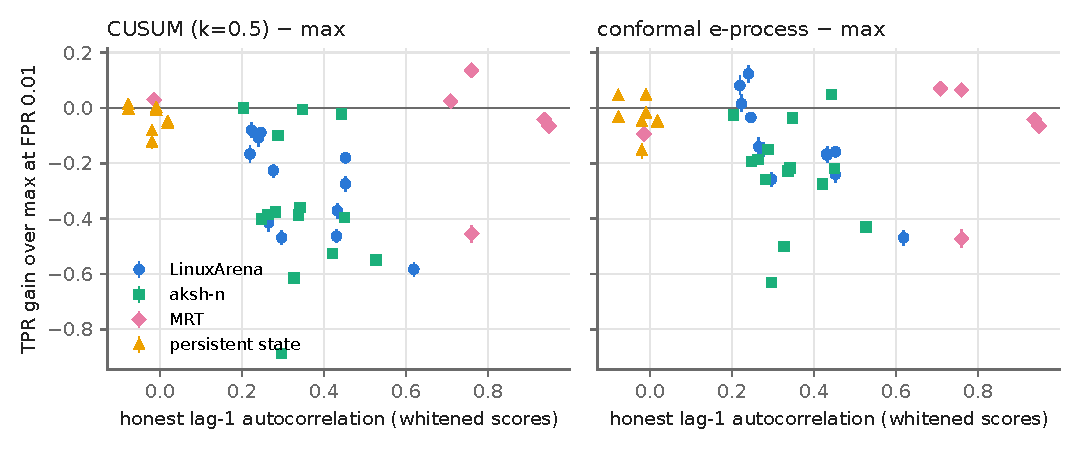
\includegraphics[width=0.74\linewidth]{t1/figures/r1_gain_vs_autocorr.pdf}
\caption{Round 1: gain over max (TPR at FPR 0.01; point estimates) vs honest lag-1 autocorrelation of whitened scores, one point per stream set. Sets with strongly autocorrelated honest scores lose the most.}\label{fig:autocorr}
\end{figure}

\subsection{1B: controlled history experiment on MonitoringBench}

Same monitor (\texttt{gpt-4.1-mini}); the history mode differs (\texttt{full} vs \texttt{none}). Table~\ref{tab:r2} gives TPR with realized FPR.

\begin{table}[!htbp]\centering\small
\begin{adjustbox}{max width=\linewidth}\begin{tabular}{@{}lcccccccc@{}}
\toprule
& \multicolumn{4}{c}{$\alpha=0.05$} & \multicolumn{4}{c}{$\alpha=0.01$}\\
\cmidrule(lr){2-5}\cmidrule(l){6-9}
Detector & full & (FPR) & none & (FPR) & full & (FPR) & none & (FPR)\\
\midrule
max & 0.226 & 0.054 & \textbf{0.322} & 0.047 & 0.171 & 0.019 & 0.156 & 0.014\\
2nd-max & \textbf{0.342} & 0.044 & 0.276 & 0.047 & 0.190 & 0.008 & 0.152 & 0.008\\
top-3 sum & 0.324 & 0.060 & 0.304 & 0.051 & \textbf{0.195} & 0.008 & \textbf{0.190} & 0.009\\
CUSUM $k{=}0.5$ & 0.073 & 0.054 & 0.087 & 0.057 & 0.030 & 0.013 & 0.039 & 0.023\\
e-process (power) & 0.130 & 0.049 & 0.127 & 0.048 & 0.052 & 0.011 & 0.065 & 0.016\\
length-aware max & 0.215 & 0.053 & 0.279 & 0.045 & 0.153 & 0.015 & 0.124 & 0.009\\
OR(max+CUSUM) & 0.201 & 0.062 & 0.247 & 0.059 & 0.137 & 0.014 & 0.086 & 0.013\\
\bottomrule
\end{tabular}\end{adjustbox}
\caption{TPR at matched trajectory FPR with realized held-out FPR, 775 attacks vs 550 honest, original prompts (\texttt{ctrl-basic-v1}). Source: \nolinkurl{results/fixes/t1/m1_realized_fpr.csv}; full detector list in \nolinkurl{results/t1/tables/r2_main.md}.}\label{tab:r2}
\end{table}

\paragraph{Corrected gains (original prompts).}\src{results/fixes/t1/gains_r2mb_corrected.csv} With history (\texttt{full}), 2nd-max and top-3 sum beat max at $\alpha=0.05$ ($+0.116$ [$+0.026$, $+0.183$]; $+0.098$ [$+0.042$, $+0.156$]), but not at $\alpha=0.01$ (top-3 sum $+0.024$ [$\m0.025$, $+0.085$], \vdrop\ relative to the earlier [0.018, 0.031]). Without history, no accumulator beats max at any $\alpha$. CUSUM $k{=}0.5$, the e-process, length-aware max and the OR chart lose to max in every cell (e.g.\ CUSUM full, $\alpha=0.01$: $\m0.141$ [$\m0.175$, $\m0.101$]). The weak history-free monitor (\texttt{gpt-4.1-nano}) is the exception: top-3 sum 0.082 vs max 0.056 at $\alpha=0.01$, gain $+0.026$ [$+0.001$, $+0.058$] (\vhold, barely).

\paragraph{The pre-registered test (original prompts).} Difference-in-differences (none $-$ full) of the gain over max: CUSUM at $\alpha=0.01$ $+0.024$ [$\m0.050$, $+0.072$] (all) and $+0.029$ [$\m0.048$, $+0.090$] (S4), both not significant. At $\alpha=0.05$ the DiD is significantly \emph{negative} for 2nd-max ($\m0.162$ [$\m0.236$, $\m0.056$]), top-3 sum ($\m0.116$ [$\m0.184$, $\m0.041$]) and CUSUM ($\m0.083$ [$\m0.161$, $\m0.004$]).\src{results/fixes/t1/did_r2mb_corrected.csv} That looked like ``accumulators gain more with history'', but the next subsection shows it was produced by the prompts.

\subsubsection{Matched prompts remove the history effect (audit M4)}\label{sec:m4}
The \texttt{full} prompt told the monitor that continuing or completing earlier suspicious activity ``counts as evidence''; the \texttt{none} prompt told it to score low even if an action could be part of a larger plan. The re-flagging mechanism proposed in round 1 is exactly what the \texttt{full} instruction asks for. We re-scored 200 Honest-550 runs and 175 attacks (100 S4 + 25 each of S1--S3) with \texttt{ctrl-matched-v1}: identical instructions, only the previous-actions block differs (21{,}786 calls, \$25.31).

\begin{table}[!htbp]\centering\small
\begin{adjustbox}{max width=\linewidth}\begin{tabular}{@{}llccc@{}}
\toprule
$\alpha$ & Detector & DiD, original prompts & DiD, matched prompts & instruction effect (orig $-$ matched)\\
\midrule
0.05 & 2nd-max & $\m0.153$ [$\m0.245$, $\m0.019$] & $\m0.023$ [$\m0.180$, $+0.090$] & $\m0.130$ [$\m0.250$, $+0.064$]\\
0.05 & top-3 sum & $\m0.122$ [$\m0.196$, $+0.003$] & $+0.030$ [$\m0.110$, $+0.123$] & $\m0.152$ [$\m0.245$, $+0.035$]\\
0.05 & CUSUM $k{=}0.5$ & $\m0.091$ [$\m0.163$, $+0.029$] & $+0.089$ [$\m0.040$, $+0.201$] & $\m0.180$ [$\m0.289$, $\m0.025$]\\
0.01 & 2nd-max & $\m0.001$ [$\m0.194$, $+0.086$] & $\m0.090$ [$\m0.210$, $+0.037$] & $+0.089$ [$\m0.107$, $+0.173$]\\
0.01 & top-3 sum & $+0.063$ [$\m0.119$, $+0.116$] & $\m0.082$ [$\m0.164$, $+0.049$] & $+0.145$ [$\m0.063$, $+0.190$]\\
0.01 & CUSUM $k{=}0.5$ & $+0.021$ [$\m0.130$, $+0.073$] & $+0.068$ [$\m0.017$, $+0.149$] & $\m0.047$ [$\m0.201$, $+0.014$]\\
\bottomrule
\end{tabular}\end{adjustbox}
\caption{DiD (none $-$ full) of the gain over max on the 200 / 175 subset, all attacks. Positive = accumulation gains concentrate in history-free mode. Source: \nolinkurl{results/fixes/t1/m4_tables.md}.}\label{tab:m4}
\end{table}

\begin{itemize}
\item On the same subset the original prompts reproduce the negative DiD at $\alpha=0.05$; with matched prompts it vanishes. ``Accumulators gain more with history'' was an \textbf{instruction artifact} (\vdrop).
\item ``Gains concentrate in history-free mode'' is still \textbf{not supported}: no matched DiD is significantly positive.
\item History-free max is \emph{lower}, not higher, with matched prompts: none $-$ full max TPR at $\alpha=0.05$ is $\m0.091$ [$\m0.186$, $+0.038$] vs $+0.089$ [$\m0.014$, $+0.159$] with the original prompts (\vrev). The original \texttt{none} instruction helped the history-free monitor.\src{results/fixes/corrections.csv (M4)}
\item Re-flagging: share of attacks with $\ge2$ steps above the honest q95, full $-$ none: all $+0.03$ [$\m0.03$, $+0.09$], S1 $+0.08$ [$\m0.08$, $+0.24$] (matched; \vweak).\src{results/fixes/t1/m4_mechanism_repeat_share.csv}
\end{itemize}

\begin{figure}[!htbp]\centering
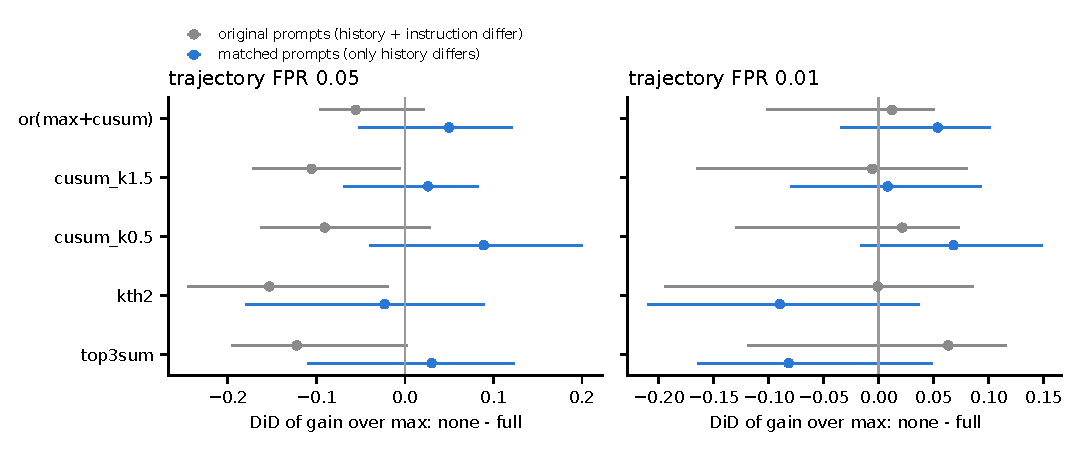
\includegraphics[width=0.76\linewidth]{fixes/t1/fig_m4_did.pdf}
\caption{DiD (none $-$ full) of the gain over max, original prompts (grey; history + instruction differ) vs matched prompts (blue; only history differs), with corrected joint task-cluster bootstrap CIs.}\label{fig:m4}
\end{figure}

\subsubsection{Agent-model confound in absolute TPR (audit M9)}\label{sec:m9}
Honest-550 is 100\% claude-opus-4-5, while 281 of the 775 attacks (36\%) are claude-opus-4-6. Max TPR at $\alpha=0.01$: opus-4-5 attacks 0.121 [0.094, 0.165] (full) / 0.117 [0.083, 0.210] (none); opus-4-6 0.258 [0.200, 0.316] / 0.224 [0.163, 0.325]. Like-for-like detection is therefore about 12\%, not ``17--20\%''. Top-3 sum on opus-4-5 attacks: 0.161 [0.093, 0.241] (full), 0.148 [0.081, 0.218] (none). Detector comparisons are paired and less affected.\src{results/fixes/t1/m9_tpr_by_agent_model.csv}

\subsection{1C: robustness (\$0)}

\begin{table}[!htbp]\centering\small
\begin{adjustbox}{max width=\linewidth}\begin{tabular}{@{}lcccc@{}}
\toprule
Detector ($\alpha=0.01$) & TPR (full) & realized FPR & TPR (none) & realized FPR\\
\midrule
max & 0.164 & 0.010 & 0.146 & 0.013\\
CUSUM $k=0.25$ & 0.024 & 0.020 & 0.031 & 0.028\\
CUSUM $k=0.5$ & 0.032 & 0.020 & 0.043 & 0.032\\
CUSUM $k=1$ & 0.097 & 0.026 & 0.070 & 0.027\\
CUSUM $k=1.5$ & \textbf{0.186} & 0.009 & 0.155 & 0.015\\
CUSUM $k=2$ & 0.162 & 0.006 & \textbf{0.159} & 0.014\\
top-2 / top-3 / top-5 sum & 0.185 / 0.205 / 0.169 & 0.011--0.013 & 0.198 / 0.186 / 0.149 & 0.009--0.016\\
GLR $W=5/10/20$ & 0.144 / 0.083 / 0.058 & 0.021--0.025 & 0.088 / 0.063 / 0.057 & 0.017--0.030\\
\bottomrule
\end{tabular}\end{adjustbox}
\caption{MonitoringBench parameter grid (775 attacks, original prompts). Source: \nolinkurl{results/t1/round3/robust/matched_kgrid_\{full,none\}.csv}.}
\end{table}

\begin{itemize}
\item \textbf{$k$ is critical.} Small-$k$ CUSUM accumulates honest noise on whitened LLM scores and also over-alarms (realized FPR 0.020--0.032 at $\alpha=0.01$). $k\approx1.5$--2 turns CUSUM into a smoothed max and recovers max-level TPR. Part of the poor showing of CUSUM $k{=}0.5$, SR and long-window GLR is mis-tuning.
\item \textbf{Dependence breaks i.i.d.\ guarantees.} The Ville ($1/\alpha$) threshold of the e-process over-alarms at about $2\times$ nominal on dependent honest streams; the analytic length-aware threshold holds nominal FPR.\src{EXPERIMENT_LOG.md (2026-10-20 T1 results, Round 3)}
\item Conformal thresholds give the same ranking; keeping the submit step changes nothing; Mondrian per-task whitening inflates FPR under grouped splits (inconclusive).
\end{itemize}

\section{Round 2: cross-session accumulation across monitors, MOLE, rule chooser}

\subsection{Persistent state re-scored by four monitors}\label{sec:ps}
All 691 runs were re-scored from the full diffs (the processed data had kept 3k of a median 39k characters) with the paper's PR-review prompt in two modes that share an identical system prompt and differ only by the previous-diffs block, so the M4 confound does not apply here.\src{results/fixes/corrections.csv (M4, persistent state row)} Paired sets: 155 honest / 120 gradual / 397 positional runs, 20 splits.

\begin{table}[!htbp]\centering\small
\begin{adjustbox}{max width=\linewidth}\begin{tabular}{@{}lccccccc@{}}
\toprule
History-free monitor & max & top-3 & top-3 $-$ max [95\% CI] & $p(\le0)$ & app-cluster & DiD (free $-$ aware) & verdict\\
\midrule
gpt-4.1-mini & 0.59 & 0.73 & $+0.145$ [$\m0.001$, $+0.228$] & 0.026 & [$\m0.016$, $+0.246$] & $\m0.169$ [$\m0.368$, $\m0.019$] & \vweak\\
GPT-4o (original scores) & 0.15 & 0.26 & $+0.101$ [$+0.015$, $+0.208$] & 0.015 & [$+0.005$, $+0.228$] & $+0.173$ [$+0.055$, $+0.271$] & \vhold\\
Gemini 2.5 Flash & 0.23 & 0.25 & $+0.021$ [$\m0.068$, $+0.101$] & 0.346 & [$\m0.077$, $+0.139$] & $\m0.028$ [$\m0.182$, $+0.091$] & \vdrop\\
Qwen3-235B-2507 & 0.44 & 0.42 & $\m0.025$ [$\m0.121$, $+0.061$] & 0.724 & [$\m0.133$, $+0.116$] & $+0.127$ [$\m0.040$, $+0.244$] & \vdrop\\
\bottomrule
\end{tabular}\end{adjustbox}
\caption{Gradual (multi-PR) attacks, run-level FPR 0.05. TPRs: \nolinkurl{results/r2_t1/ps_tables.md}; corrected gains and DiDs: \nolinkurl{results/fixes/r2_t1/ps_gains_corrected.csv}, \nolinkurl{results/fixes/r2_t1/ps_did_corrected.csv}, \nolinkurl{results/fixes/corrections.csv}. The GPT-4o row uses the paired filter (153 honest), hence $+0.101$ rather than the round-1 $+0.146$.}\label{tab:ps}
\end{table}

\begin{itemize}
\item \textbf{The history-free gain is monitor-specific.} It holds for GPT-4o, is borderline for gpt-4.1-mini ($p(\le0)=0.026$; CI touches 0), and is absent for Gemini and Qwen. At FPR 0.01 none of the earlier gains survive: gpt-4.1-mini SR $+0.063$ [$\m0.003$, $+0.170$], Gemini top-3 $+0.043$ [$\m0.051$, $+0.156$] (both \vdrop).
\item \textbf{Side-task success.} 66 of 120 gradual attacks failed their side task. gpt-4.1-mini on successful attacks ($n=54$): $+0.241$ [$+0.073$, $+0.336$]; failed: $+0.067$ [$\m0.067$, $+0.187$]. GPT-4o on successful attacks: $+0.051$ [$\m0.053$, $+0.164$]; its pooled gain comes from failed attacks ($+0.142$ [$+0.020$, $+0.269$]).\src{results/fixes/corrections.csv (m9)}
\item \textbf{``History kills the gain'' holds for one monitor of four.} The DiD is significantly positive only for GPT-4o; Qwen's is not significant; gpt-4.1-mini's is significantly the other way. With all prior diffs, gpt-4.1-mini keeps re-flagging gradual attacks while honest PRs stay low: its max drops to 0.35 and top-3 sum gains $+0.315$ [$+0.156$, $+0.443$] over that weak max.\src{results/fixes/r2_t1/ps_gains_corrected.csv}
\item \textbf{Positional (single-PR) attacks:} max is best for every new monitor (gpt-4.1-mini top-3 $-$ max $\m0.164$ [$\m0.284$, $\m0.058$]).
\item Only 5-PR sequences with matching honest runs exist, so longer horizons were tested by streaming over concatenated honest prefixes (\S\ref{sec:longh}), not by longer attacks.
\end{itemize}

\subsection{MOLE, round 2 (two corpora)}
History-free gpt-4.1-mini account-day monitor (MOLE judge prompt and taxonomy) plus MOLE's z-score and peer-fit, 30 workdays, account-level FPR 0.10. Corrected gains:\src{results/fixes/corrections.csv (C2, MOLE rows)}
\begin{itemize}
\item GPT-5.3 single-day (30 insiders, 3--4 attack days each), LLM 3rd-max $-$ max: $+0.131$ [$\m0.028$, $+0.287$], $p(\le0)=0.058$; top-4 sum $+0.086$ [$\m0.021$, $+0.218$]; at FPR 0.05: $+0.088$ [$\m0.045$, $+0.259$]. All \textbf{not significant} (previously $+0.131$ [0.11, 0.15]).
\item Peer-fit 3rd-max: $+0.172$ [$+0.042$, $+0.317$] (significant on this corpus).
\item GPT-5.3 multiday (one attack day): $\m0.172$ [$\m0.298$, $+0.041$]. DeepSeek-V4 single-day: $\m0.039$ [$\m0.209$, $+0.129$].
\item Accumulators alarm 7--15 workdays later than max. Under MOLE's daily top-$K$ review budget, today's score is best: R@10/day 0.395 for today's gpt-4.1-mini score (MOLE's reported 0.244), vs 0.28 for the running max and 0.31 for the top-3 sum.\src{results/r2_t1/mole_tables.md}
\end{itemize}

\subsection{Out-of-sample rule chooser (67 sets)}
The 67 sets are the 46 round-1 sets (existing streams and MonitoringBench variants), 12 new persistent-state sets and 9 MOLE sets. The chooser sees the honest calibration half plus $n_\text{lab}=20$ labeled attacks. Round 2 reported $+0.023$ [0.012, 0.038] for the empirical chooser at FPR 0.01. That number is a winner's curse: the chosen rules over-alarmed (realized FPR 0.0156 vs 0.0142 for always-max), because selecting the rule with the best labeled-attack TPR at its own threshold favours rules whose threshold is low by calibration noise (audit M6).

\begin{table}[!htbp]\centering\small
\begin{adjustbox}{max width=\linewidth}\begin{tabular}{@{}lccc@{}}
\toprule
Chooser (gain over always-max, FPR 0.01) & same calibration (round 2) & nested & FPR-matched\\
\midrule
empirical, 20 labels & $+0.023$ [$+0.011$, $+0.035$] & $+0.001$ [$\m0.014$, $+0.013$] & $+0.009$ [$\m0.003$, $+0.023$]\\
empirical, 40 labels & $+0.026$ [$+0.015$, $+0.038$] & $\m0.001$ [$\m0.013$, $+0.009$] & $+0.009$ [$\m0.006$, $+0.024$]\\
LOSO ridge meta-chooser & $+0.019$ [$+0.007$, $+0.032$] & $\m0.006$ [$\m0.021$, $+0.006$] & $+0.007$ [$\m0.007$, $+0.025$]\\
mechanism rule & $\m0.022$ [$\m0.049$, $+0.005$] & $\m0.017$ [$\m0.047$, $+0.009$] & $\m0.018$ [$\m0.042$, $+0.010$]\\
empirical, FPR 0.05 & $+0.014$ [$0.005$, $0.028$] & $+0.004$ [$\m0.010$, $+0.014$] & $+0.007$ [$\m0.005$, $+0.016$]\\
\bottomrule
\end{tabular}\end{adjustbox}
\caption{Rule chooser, 95\% CIs from a cluster bootstrap over 14 set families; task-grouped labeled draw. Source: \nolinkurl{results/fixes/corrections.csv} (M6, M7), \nolinkurl{results/fixes/r2_t1/chooser_fixed_summary_task_lab20.csv}.}\label{tab:chooser}
\end{table}

\begin{figure}[!htbp]\centering
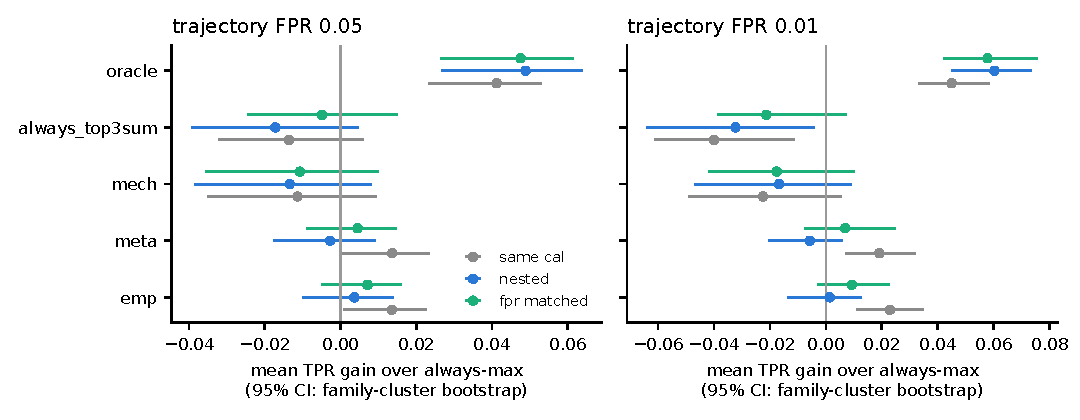
\includegraphics[width=0.76\linewidth]{fixes/r2_t1/fig_chooser_fixed_task_lab20.pdf}
\caption{Mean TPR gain over always-max for the chooser variants under same-calibration (grey), nested (blue) and FPR-matched (green) evaluation, 95\% family-cluster CIs. Only the oracle (which sees the test attacks) stays above zero.}\label{fig:chooser}
\end{figure}

Once selection noise is separated from threshold noise, no chooser beats always-max (\vdrop). The ``always top-3 sum'' policy loses ($\m0.032$ nested, family CI [$\m0.064$, $\m0.004$]), and CUSUM with $k$ tuned on the labeled attacks loses $\m0.051$ [$\m0.092$, $\m0.023$] nested.\src{results/fixes/r2_t1/chooser_fixed_summary_task_lab20.csv}

\paragraph{Length-aware + top-$k$ hybrid (negative, holds).} Length-tercile conformal calibration of top-3 sum loses $\m0.152$ [$\m0.243$, $\m0.040$] (family CI) at FPR 0.01; per-set significant losses fall from 36/46 to 19/46 under corrected CIs. The analytic length-aware max remains the only length fix that helps, and only where lengths differ.\src{results/fixes/r2_t1/hybrid_summary_corrected.csv}

\subsection{Mechanism correlations are descriptive}\label{sec:mech}
Round 1 reported that the top-3 gain tracks the repeat-spike likelihood ratio (Spearman $+0.47$, 46 sets) and that the CUSUM gain falls with honest spike persistence ($\m0.67$). Those correlations computed the predictor from the same attacks that define the gain and treated correlated sets (full/none, local/cumulative, integer/expected copies) as independent (audit M7). With the predictor estimated on disjoint labeled attacks across 67 sets:\src{results/fixes/r2_t1/chooser_mechanism_task_lab20.csv}
\begin{itemize}
\item top-3 sum gain vs repeat-spike LR: $+0.30$ (naive $p$ 0.013), family-cluster CI [$\m0.03$, $+0.45$]; family means $+0.28$ ($p$ 0.33) (\vweak);
\item CUSUM $k{=}0.5$ gain vs honest persistence: $\m0.56$, family CI [$\m0.69$, $\m0.05$] at FPR 0.05 (same calibration); under FPR matching [$\m0.73$, $+0.02$]; family means $\m0.39$ ($p$ 0.16). Directionally consistent, not robust.
\end{itemize}
The rule built on these properties loses to always-max (Table~\ref{tab:chooser}), so ``choose the rule from stream properties'' is \vdrop.

\section{Round 3: accumulation at scale and re-flagging designs}

All round-3 gains use the corrected paired bootstrap, nested choosers and reported realized FPR. Pre-specified comparisons: 3rd-max, top-3 sum, CUSUM $k{=}1.5$ and the chooser vs max. The round-2 MOLE corpora are ``discovery''; the five new corpora are ``confirmation''.\src{EXPERIMENT_LOG.md (2026-10-22 r3t1 entry)}

\subsection{MOLE: all eight corpora with one common monitor}
The common monitor is a history-free Qwen3-235B-2507 account-day judge (MOLE prompt and taxonomy, compact audit rendering, integer score). Robustness monitors: gpt-4.1-mini with full rendering (GPT-5.3 corpora), MOLE z-score and peer-fit, an activity-only baseline (log events per day) and account-centered variants.

\begin{table}[!htbp]\centering\small
\begin{adjustbox}{max width=\linewidth}\begin{tabular}{@{}lcccccc@{}}
\toprule
Corpus & $n_h/n_a$ & max TPR & 3rd-max $-$ max & top-3 sum $-$ max & CUSUM $k{=}1.5$ $-$ max & nested chooser\\
\midrule
GPT-5.3 single-day & 112/30 & 0.38 & $\m0.021$ [$\m0.15$, $+0.09$] & $\m0.044$ [$\m0.15$, $+0.04$] & $+0.012$ [$\m0.06$, $+0.08$] & $\m0.026$\\
DeepSeek-V4 single-day & 112/30 & 0.31 & $+0.014$ [$\m0.11$, $+0.13$] & $+0.077$ [$\m0.08$, $+0.25$] & $\m0.059$ [$\m0.17$, $+0.07$] & $+0.030$\\
Qwen3.6-27B single-day & 112/30 & 0.38 & $\m0.174$ [$\m0.36$, $\m0.02$] & $\m0.085$ [$\m0.25$, $+0.04$] & $\m0.079$ [$\m0.16$, $+0.03$] & $\m0.039$\\
Kimi-K2.6 single-day & 112/30 & 0.30 & $\m0.157$ [$\m0.31$, $+0.03$] & $\m0.096$ [$\m0.22$, $+0.06$] & $\m0.037$ [$\m0.10$, $+0.06$] & $\m0.016$\\
GPT-5.3 multiday & 112/38 & 0.35 & $\m0.187$ [$\m0.33$, $\m0.05$] & $\m0.073$ [$\m0.19$, $+0.07$] & $\m0.004$ [$\m0.08$, $+0.05$] & $\m0.084$\\
DeepSeek-V4 multiday & 114/36 & 0.18 & $+0.070$ [$\m0.05$, $+0.18$] & $+0.052$ [$\m0.07$, $+0.20$] & $+0.065$ [$\m0.05$, $+0.20$] & $+0.023$\\
Qwen3.6-27B multiday & 113/37 & 0.23 & $\m0.067$ [$\m0.19$, $+0.04$] & $\m0.022$ [$\m0.12$, $+0.07$] & $\m0.081$ [$\m0.14$, $\m0.01$] & $\m0.011$\\
Kimi-K2.6 multiday & 114/36 & 0.17 & $\m0.074$ [$\m0.19$, $+0.04$] & $\m0.035$ [$\m0.13$, $+0.08$] & $\m0.018$ [$\m0.08$, $+0.07$] & $\m0.031$\\
\midrule
Pooled single-day (RE) & & & $\m0.066$ [$\m0.156$, $+0.023$] & $\m0.045$ [$\m0.109$, $+0.019$] & $\m0.030$ [$\m0.073$, $+0.013$] & \\
Pooled multiday (RE) & & & $\m0.060$ [$\m0.160$, $+0.039$] & $\m0.022$ [$\m0.078$, $+0.034$] & $\m0.022$ [$\m0.073$, $+0.030$] & \\
\bottomrule
\end{tabular}\end{adjustbox}
\caption{Common monitor (Qwen3-235B, integer score), account-level FPR 0.10, paired gains with corrected CIs; realized FPR of max 0.096--0.114. Pooled rows: random-effects meta-analysis over 4 corpora. Source: \nolinkurl{results/r3_t1/mole_tables.md}.}\label{tab:mole}
\end{table}

\begin{figure}[!htbp]\centering
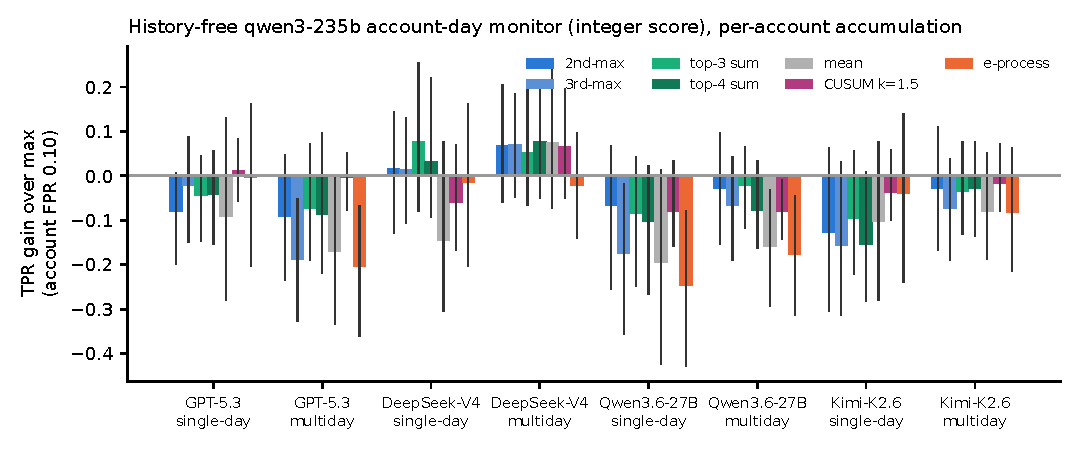
\includegraphics[width=0.82\linewidth]{r3_t1/fig_mole_gain_by_corpus.pdf}
\caption{Gain over max at account FPR 0.10 for every accumulator, common monitor, all eight corpora (corrected paired-bootstrap CIs).}\label{fig:mole}
\end{figure}

\begin{itemize}
\item \textbf{No accumulation rule beats max on any corpus} (no significantly positive gain in Table~\ref{tab:mole}; significant losses on three cells). Mean is worse still (pooled single-day $\m0.130$ [$\m0.229$, $\m0.031$]). The nested chooser stays with max in most splits. Audit 2 reproduced the pooled single-day 3rd-max estimate ($\m0.073$ [$\m0.166$, $+0.019$]).\src{results/audit2/repro_mole.csv}
\item \textbf{Provider mix (audit 2, m7).} DeepSeek single-day was scored by a mix of Qwen3-235B providers clustered by account; the logprob provider scores routine days about one point higher. Dropping those accounts: DeepSeek 3rd-max $-$ max $\m0.012$, pooled single-day $\m0.064$ [$\m0.131$, $+0.003$]. Conclusion unchanged.\src{results/audit2/repro_mole_provider.csv}
\item \textbf{Horizon sweep} (first 5/10/15/20 workdays, GPT-5.3 single-day, common monitor): no horizon gives a gain above $+0.06$. Order-statistic rules lose 0.08--0.18 at 5--10 days; at 15--20 days all gains lie between $\m0.11$ and $+0.05$; CUSUM $k{=}1.5$ stays within $\pm0.01$ (point estimates).\src{results/r3_t1/mole_tables.md (horizon sweep)}
\item \textbf{Daily review budget} (MOLE's R@10/day): today's score is best or within 0.01 of the best on 9 of 11 corpus$\times$monitor cells (today: 0.15--0.43). Exceptions: Kimi single-day (running max 0.18 vs today 0.15) and gpt-4.1-mini on GPT-5.3 multiday (CUSUM $k{=}1.5$ 0.46 vs 0.43). 3rd-max and top-3 sum are worse everywhere.\src{results/r3_t1/mole_tables.md (daily review budget)}
\end{itemize}

\paragraph{The round-2 MOLE gain is not robust.} Insider accounts are slightly more active (median events per day 123 on other days vs 116 routine on GPT-5.3 single-day), and the round-2 monitor separates them on non-attack days too (day AUROC 0.65).

\begin{table}[!htbp]\centering\small
\begin{adjustbox}{max width=\linewidth}\begin{tabular}{@{}lcccc@{}}
\toprule
Monitor (GPT-5.3 single-day) & max TPR & 3rd-max $-$ max & account-centered & without attack days\\
\midrule
gpt-4.1-mini (round-2 monitor) & 0.31 & $+0.126$ [$\m0.019$, $+0.259$] & $\m0.001$ [$\m0.174$, $+0.126$] & $+0.048$ [$\m0.058$, $+0.175$] (max 0.125)\\
Qwen3-235B (common) & 0.38 & $\m0.021$ [$\m0.15$, $+0.09$] & $\m0.027$ [$\m0.15$, $+0.07$] & $\m0.025$\\
peer-fit & 0.17 & $+0.172$ [$+0.04$, $+0.31$] & $+0.139$ [$+0.01$, $+0.33$] & $+0.123$\\
activity only (no content) & 0.00 & $+0.320$ [$+0.14$, $+0.49$] & $+0.178$ [$+0.06$, $+0.31$] & $+0.232$\\
\bottomrule
\end{tabular}\end{adjustbox}
\caption{Account-level confound checks at FPR 0.10. gpt-4.1-mini row: audit-2 reproduction (\nolinkurl{results/audit2/corrections.csv}, m5); other rows: \nolinkurl{results/r3_t1/mole_tables.md}. The activity-only gain is over a degenerate max (TPR 0.00).}\label{tab:moleconf}
\end{table}

The gpt-4.1-mini gain was not significant to begin with and vanishes after account centering; without attack days that monitor barely separates insider accounts (max TPR 0.125). The data cannot separate an account-level confound from noise, so the correct statement is that \textbf{the round-2 MOLE gain is not robust}.\src{results/audit2/corrections.csv (m5)} An activity-only ``monitor'' with no content reaches 3rd-max TPR 0.32 (the log's ``0.37'' was a typo; audit 2, m6). Peer-fit keeps a significant gain on GPT-5.3 single-day even after centering, but this does not replicate: pooled over the four single-day corpora peer-fit 3rd-max is $+0.022$ [$\m0.097$, $+0.142$].\src{results/r3_t1/mole_tables.md (meta-analysis)}

\paragraph{Mechanism (audit 2, A3).} Across 64 corpus$\times$monitor cells the top-3 gain correlates with repeat-spike informativeness, Spearman $+0.297$ (naive $p$ 0.017). The cells are 8 corpora $\times$ up to 10 dependent monitor variants (centered copies, activity baseline), and the predictor comes from the same insider streams. Corpus-cluster 95\% CI [$\m0.04$, $+0.54$]; primary monitors only (29 cells) $+0.18$ ($p$ 0.36). Descriptive only (\vweak).\src{results/audit2/corrections.csv (A3)} For the common monitor on single-day corpora, a repeat high day is barely more likely for insiders than for routine accounts (repeat-spike log-LR $\m0.02$ on GPT-5.3 single-day) while honest persistence is high (0.47).\src{results/r3_t1/mole_tables.md (per-corpus stream features)}


\subsection{Persistent state under continuous monitoring (no reset)}\label{sec:longh}
Attack runs are appended after 0--4 random honest test runs; thresholds are set for a matched in-control ARL$_0=5/\alpha$ PRs; detection means an alarm inside the attack run given no prefix alarm. No attack longer than 5 PRs was built: concatenating independent runs would fabricate cross-run continuity that no agent produced.

\begin{table}[!htbp]\centering\small
\begin{adjustbox}{max width=\linewidth}\begin{tabular}{@{}lcccccc@{}}
\toprule
Set (\texttt{current\_only}) & ARL$_0$ target & max (realized ARL$_0$) & CUSUM $k{=}0.5$ (realized ARL$_0$) & CUSUM $k{=}1.5$ & 2nd-max & top-3 sum\\
\midrule
gpt-4.1-mini, gradual & 100 & 0.58 (102) & \textbf{0.71} (107) & 0.67 & 0.04 & 0.00\\
gpt-4.1-mini, gradual & 500 & 0.48 (no honest alarm) & \textbf{0.59} (661) & 0.54 & 0.04 & 0.00\\
gpt-4.1-mini, positional & 100 & \textbf{0.65} & 0.49 & 0.65 & 0.01 & 0.00\\
gpt-4.1-mini, positional & 500 & 0.56 & 0.19 & \textbf{0.57} & 0.01 & 0.00\\
GPT-4o (original), gradual & 100 & 0.16 (120) & \textbf{0.27} (106) & 0.16 & 0.00 & 0.00\\
GPT-4o (original), gradual & 500 & 0.01 (no honest alarm) & \textbf{0.19} (2{,}387) & 0.01 & 0.00 & 0.00\\
\bottomrule
\end{tabular}\end{adjustbox}
\caption{Detection rate under continuous monitoring. Sources: \nolinkurl{results/r3_t1/ps_longhorizon.md}, \nolinkurl{results/r3_t1/ps_longhorizon_arl.csv}. No CIs were computed. ``No honest alarm'': the integer-score max threshold never fired on the honest test stream, so its realized ARL$_0$ is unresolved.}\label{tab:longh}
\end{table}

\begin{itemize}
\item For history-free gpt-4.1-mini on gradual attacks, CUSUM $k{=}0.5$ beats max: 0.71 vs 0.58 at ARL$_0=100$ PRs (realized ARL$_0$ 107 vs 102) and 0.59 vs 0.48 at 500. GPT-4o: 0.27 vs 0.16 at 100.
\item On positional (single-PR) attacks, CUSUM $k{=}0.5$ loses (0.49 vs 0.65); $k{=}1.5$ matches max.
\item Non-forgetting accumulators (k-th largest, top-$k$ sum over the whole stream) collapse to $\approx0$. In deployment, cross-session accumulation has to forget (CUSUM) or be windowed.
\item Caveats: point estimates without CIs; at ARL$_0=500$ the max threshold is not matched; Gemini and Qwen streams give low or mixed detection (Gemini history-free $\le0.14$ for every rule).
\end{itemize}

\subsection{Re-flagging as a monitor design target}
Round 2 suggested that what helps accumulation is attack re-flagging (a high repeat-spike LR), not history per se. Round 3 tested monitor designs that target it, all with gpt-4.1-mini, as matched pairs differing only in the variable under test: \emph{history-free}; \emph{history-aware} (plain); \emph{reflag} = history-aware + an explicit rule to re-raise suspicion when the current unit continues earlier suspicious work; \emph{ledger} = no history but the monitor's own ledger of open suspicions, with a \emph{ledger-null} control (identical prompt, notes always empty); two samples at $T=1$ (each alone, their mean, or both as separate units).

\begin{table}[!htbp]\centering\small
\begin{adjustbox}{max width=\linewidth}\begin{tabular}{@{}lcccccc@{}}
\toprule
Design & run-max AUROC & repeat-spike log-LR & max @0.05 & top-3 @0.05 (gain over max) & max @0.01 & top-3 @0.01 (gain)\\
\midrule
history-free & 0.897 & $+1.90$ & 0.58 & \textbf{0.74} ($+0.16$ [$+0.02$, $+0.23$]) & 0.50 & 0.53 ($+0.03$ [$\m0.03$, $+0.22$])\\
history-aware & 0.831 & $+1.91$ & 0.37 & 0.67 ($+0.30$ [$+0.16$, $+0.42$]) & 0.21 & \textbf{0.57} ($+0.35$ [$+0.24$, $+0.44$])\\
reflag & 0.806 & $+2.00$ & 0.40 & 0.56 ($+0.16$ [$+0.05$, $+0.32$]) & 0.14 & 0.44 ($+0.30$ [$+0.12$, $+0.39$])\\
ledger & 0.856 & $+1.45$ & 0.55 & 0.64 ($+0.08$ [$\m0.03$, $+0.19$]) & 0.23 & 0.18 ($\m0.05$ [$\m0.11$, $+0.19$])\\
ledger-null & 0.860 & $+3.63$ & 0.37 & 0.58 ($+0.21$ [$+0.03$, $+0.33$]) & 0.08 & 0.27 ($+0.19$ [$+0.08$, $+0.33$])\\
sample0 ($T{=}1$) & 0.816 & $+2.90$ & 0.45 & 0.50 ($+0.05$ [$\m0.01$, $+0.22$]) & 0.26 & 0.26 ($+0.00$ [$\m0.05$, $+0.14$])\\
sample1 ($T{=}1$) & 0.858 & $+2.42$ & 0.49 & 0.63 ($+0.14$ [$+0.04$, $+0.21$]) & 0.43 & 0.52 ($+0.09$ [$+0.03$, $+0.19$])\\
sample mean & 0.868 & $+1.92$ & 0.57 & 0.72 ($+0.16$ [$+0.03$, $+0.24$]) & 0.45 & 0.45 ($+0.00$ [$\m0.05$, $+0.21$])\\
sample units & 0.838 & $+1.33$ & 0.53 & 0.66 ($+0.13$ [$+0.05$, $+0.24$]) & 0.34 & 0.51 ($+0.17$ [$+0.07$, $+0.23$])\\
length only ($-\log$ chars) & 0.585 & $+0.32$ & 0.13 & 0.28 ($+0.15$ [$+0.10$, $+0.33$]) & 0.05 & 0.16 ($+0.11$ [$+0.06$, $+0.16$])\\
\bottomrule
\end{tabular}\end{adjustbox}
\caption{Persistent state, gradual attacks (155 honest / 120 attack), run-level FPR 0.05 and 0.01; top-3 sum on whitened scores; corrected paired-bootstrap CIs. Source: \nolinkurl{results/r3_t1/reflag_tables.md} (ps:gradual).}\label{tab:reflag}
\end{table}

\begin{figure}[!htbp]\centering
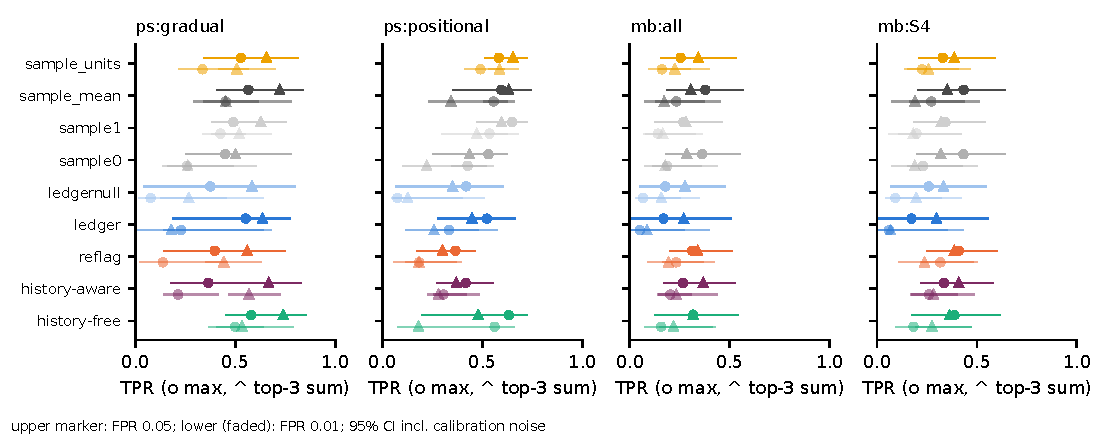
\includegraphics[width=0.8\linewidth]{r3_t1/fig_reflag_tpr.pdf}
\caption{TPR of max (o) and whitened top-3 sum ($\wedge$) per design; upper marker FPR 0.05, lower 0.01; 95\% CIs include calibration noise.}\label{fig:reflag}
\end{figure}

\begin{itemize}
\item \textbf{Re-flagging is not a better design.} The explicit reflag rule lowers run-max AUROC relative to the plain history-aware monitor (0.806 vs 0.831) and leaves the repeat-spike LR unchanged (2.00 vs 1.91). The best rule at 5\% FPR is history-free whitened top-3 sum (0.74). Audit 2 reproduced it exactly (0.742 vs 0.581, $+0.161$ [$+0.026$, $+0.233$]) but found that it depends on the whitening: with raw logprob-expected scores the top-3 sum gains only $+0.031$ [$+0.001$, $+0.070$], and at FPR 0.01 $+0.037$ [$\m0.019$, $+0.213$].\src{results/audit2/issues.csv (m8)}
\item At 1\% FPR the best rules are close with overlapping CIs: history-aware top-3 0.57, history-free top-3 0.53, history-free max 0.50.
\item \textbf{Ledger.} The carried notes raise max-type detection relative to ledger-null (0.55 vs 0.37), but the ledger monitor's honest scores grow with diff length (Spearman $+0.71$ within honest PRs), and it is not better than history-free.\src{results/r3_t1/ps_length_check.csv}
\item \textbf{Two samples.} Each $T{=}1$ sample has a weaker max than $T{=}0$ (0.45 / 0.49 vs 0.58); their mean recovers it (top-3 0.72). Using both samples as units gives a small significant accumulation gain on \emph{positional} attacks at 1\% FPR: top-3 $+0.09$ [$+0.03$, $+0.13$] over that stream's max.
\item \textbf{Nested chooser} gains $+0.05$ to $+0.31$ over max where top-$k$ clearly wins (persistent-state gradual) and stays within $\pm0.07$ of max elsewhere, at realized FPR close to nominal.
\item \textbf{MonitoringBench} (150 honest / 150 attacks): the best TPR at 5\% FPR is 0.39 on all attacks and 0.46 on S4 (history-aware 2nd-max in both); history-free max is 0.32 / 0.39. The reflag rule lowers the repeat-spike LR vs the plain history-aware prompt (0.45 vs 0.58). Gains over max reach $+0.14$ to $+0.15$ only where that design's own max is weak (ledger-null all attacks, 2nd-max $+0.14$ [$+0.06$, $+0.23$]).\src{results/r3_t1/reflag_tables.md (mb sections)}
\end{itemize}

\paragraph{Validity checks: length.} Gradual-attack diffs are about 4$\times$ shorter than honest diffs (median 13{,}427 vs 53{,}602 characters), and a length-only ``monitor'' with 2nd-max reaches TPR 0.40 at 5\% FPR. Monitor scores \emph{rise} with diff length within honest PRs (gpt-4.1-mini $+0.09$, Qwen $+0.51$, ledger $+0.71$), so length works against the monitors; it also explains Qwen's high honest persistence in round 2. Length-matched subsets (25/25) are too small to conclude anything (realized FPR $\approx0.15$). On MonitoringBench, attacks are longer (stream-length AUROC 0.72); the opus-4-5-only and length-matched subsets give the same qualitative picture.\srcs{results/r3_t1/ps_length_check.csv}{results/r3_t1/reflag_tables.md}

\section{What holds, what was weakened, what was dropped}\label{sec:verdicts}

Audit 1 found 2 critical, 9 major and 13 minor issues across all tracks; those touching Idea 1 are C2, M4, M6, M7, M8, M9, m1, m7, m9, m10, m12.\src{results/audit/issues.csv} Audit 2 re-implemented the round-3 analyses independently (randomized plug-in thresholds, task-grouped splits, a joint cluster bootstrap with thresholds recomputed); every round-3 Idea-1 headline reproduced within split and bootstrap noise, and the issues affecting this report are A3, m5, m6, m7 and m8.\src{results/audit2/issues.csv} Figure~\ref{fig:c2} shows the size of the main inference correction.

\begin{figure}[!htbp]\centering
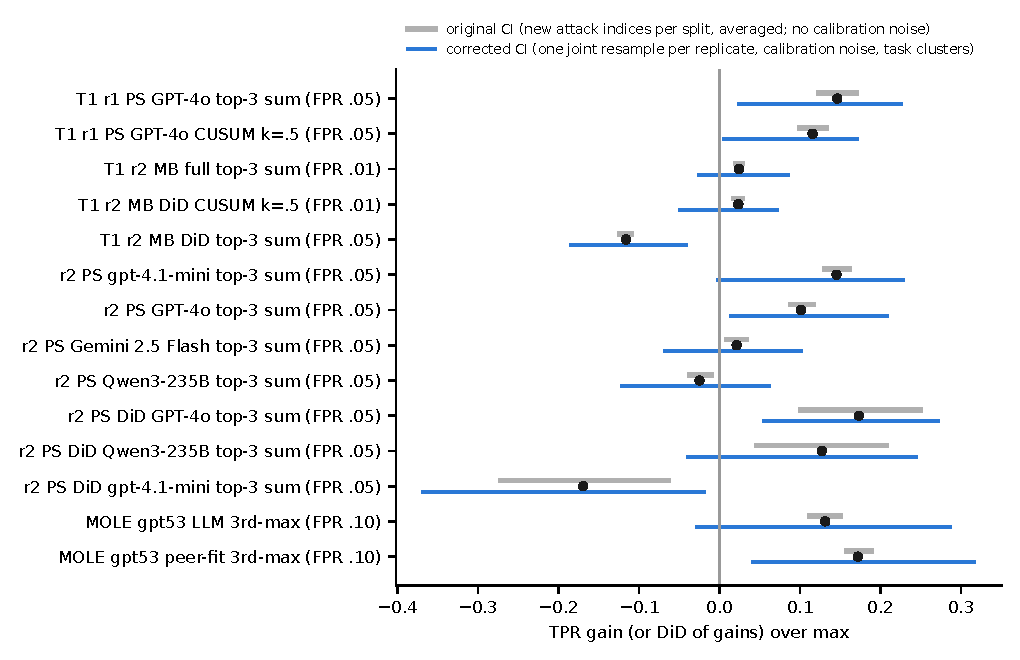
\includegraphics[width=0.62\linewidth]{fixes/t1/fig_c2_headline_cis.pdf}
\caption{Headline gains over max with the original CIs (grey; new attack indices per split, averaged; no calibration noise) and the corrected CIs (blue; one joint resample per replicate, calibration noise, task clusters).}\label{fig:c2}
\end{figure}

\subsection*{Holds}
\begin{itemize}
\item Max-type rules (max, 2nd-max, length-aware max) match or beat every accumulator on most real per-step stream sets (86\% / 67\% / 83\% of aksh-n / LinuxArena / MRT sets at FPR 0.01); textbook CUSUM $k{=}0.5$, SR, long-window GLR and e-processes lose almost everywhere.\src{results/t1/tables/r1_tpr.md}
\item Cross-session accumulation of history-free GPT-4o per-PR scores: $+0.146$ [$+0.025$, $+0.226$] (round 1), $+0.101$ [$+0.015$, $+0.208$] (paired filter); history-aware GPT-4o loses the gain (DiD $+0.173$ [$+0.055$, $+0.271$]).
\item Under continuous no-reset monitoring a forgetting accumulator beats max for history-free gpt-4.1-mini on gradual attacks (CUSUM $k{=}0.5$ 0.71 vs 0.58 at ARL$_0=100$); non-forgetting top-$k$ collapses (point estimates).
\item MOLE: no accumulation rule beats max for the common monitor on any of 8 corpora (pooled single-day 3rd-max $\m0.066$ [$\m0.156$, $+0.023$]); today's score is the best (or within 0.01 of the best) daily-review rule on 9 of 11 cells.
\item CUSUM's reference value is critical ($k\approx1.5$--2 $\approx$ max on whitened LLM scores; small $k$ over-alarms); e-process Ville thresholds over-alarm on dependent streams.
\item Length-aware max on MRT ($+0.365$ [$+0.127$, $+0.445]$), conditional on unadapted attack lengths.
\item Weak history-free monitor (gpt-4.1-nano): top-3 sum $+0.026$ [$+0.001$, $+0.058$] at FPR 0.01.
\item Length-tercile hybrid is a loss ($\m0.152$ [$\m0.243$, $\m0.040$]).
\item Positional (single-PR) attacks: max is best (gpt-4.1-mini top-3 $\m0.164$ [$\m0.284$, $\m0.058$]).
\end{itemize}

\subsection*{Weakened}
\begin{itemize}
\item History-free gpt-4.1-mini PR gain: $+0.145$ [$\m0.001$, $+0.228$], $p(\le0)=0.026$ (borderline); significant on side-task-successful attacks ($+0.241$ [$+0.073$, $+0.336$]); the round-3 whitened top-3 gain ($+0.16$ [$+0.02$, $+0.23$]) shrinks to $+0.031$ with raw scores.
\item GPT-4o CUSUM gain $+0.116$ [$+0.006$, $+0.171$]; app-cluster interval crosses zero. GPT-4o's pooled gain comes from side-task-failed attacks.
\item ``History removes the gain'': significant for 1 of 4 monitors (GPT-4o), reversed for gpt-4.1-mini.
\item Mechanism correlations (repeat-spike LR, honest persistence): descriptive; family/corpus-cluster CIs include or approach zero (67 sets: $+0.30$ [$\m0.03$, $+0.45$]; MOLE: $+0.297$ [$\m0.04$, $+0.54$]).
\item Re-flagging under history on MonitoringBench: $+0.03$ [$\m0.03$, $+0.09$] with matched prompts.
\item Absolute MonitoringBench TPR: about 12\% like-for-like (opus-4-5) at 1\% FPR; realized FPR averages 1.28$\times$ nominal at $\alpha=0.01$.
\item ``Round-2 MOLE gain was an account-level confound'': restated as not robust (never significant; vanishes after centering).
\item Max alarms at the ideal flag step: partly by construction.
\end{itemize}

\subsection*{Dropped or reversed}
\begin{itemize}
\item MonitoringBench full-mode top-3 sum gain at FPR 0.01 ($+0.024$ [$\m0.025$, $+0.085$]) and the CUSUM DiD ($+0.024$ [$\m0.050$, $+0.072$]).
\item ``Accumulators gain more with history'' (negative DiD at FPR 0.05): instruction artifact; near zero with matched prompts.
\item ``History-free max beats history-aware max'' on MonitoringBench: reversed with matched prompts ($\m0.091$ [$\m0.186$, $+0.038$]).
\item Persistent-state gains for Gemini 2.5 Flash and Qwen3-235B, and all FPR-0.01 persistent-state gains from round 2.
\item Qwen's history DiD ($+0.127$ [$\m0.040$, $+0.244$]).
\item MOLE round-2 3rd-max gain ($+0.131$ [$\m0.028$, $+0.287$]) as a positive result.
\item Rule chooser gain ($+0.023$ $\to$ $+0.001$ nested) and the practitioner lesson ``estimate stream properties, then pick the rule''.
\end{itemize}
Sources for this section: \nolinkurl{results/fixes/corrections.csv}, \nolinkurl{results/audit2/corrections.csv} and the tables cited above.

\section{Conclusions}
\begin{enumerate}
\item \textbf{Keep max as the default decision rule, with a length-aware null where honest and attack lengths differ.} At a matched budget, textbook sequential tests with default parameters lose to max-type rules on almost every per-step stream set, and no data-driven rule selection we tried beats always-max out of sample.
\item \textbf{Cross-session accumulation is the one positive regime, and it is fragile.} With a history-free per-PR monitor it helps for GPT-4o and (borderline) gpt-4.1-mini, not for Gemini or Qwen. In a deployment that monitors continuously without resets, use a forgetting statistic (CUSUM $k\approx0.5$--1.5) rather than a k-th largest or top-$k$ sum.
\item \textbf{Insider-style account monitoring does not benefit} from per-account accumulation of a content monitor across eight MOLE corpora; review today's highest-scoring account-days.
\item \textbf{The history double-counting hypothesis is not supported} on MonitoringBench, and the earlier opposite effect was an instruction artifact. Prompt wording moves detection as much as history does, so history-mode comparisons must hold the instructions fixed.
\item \textbf{If using CUSUM on LLM scores, tune $k$ to the score distribution} ($k\approx1.5$--2 on whitened scores) and calibrate thresholds empirically, reporting realized FPR.
\end{enumerate}

\section{Limitations}
\begin{itemize}
\item \textbf{Small honest sets} (112--550 per set): FPR-0.01 thresholds are noisy (realized FPR up to 2.3$\times$ nominal) and many contrasts are inconclusive rather than negative.
\item \textbf{Short cross-session sequences} (5 PRs); long-horizon results splice honest prefixes before 5-PR attacks and have no CIs.
\item \textbf{Label and surface confounds.} MonitoringBench agent-model mismatch (honest all opus-4-5); persistent-state diff length (attacks 4$\times$ shorter); MOLE insider activity; side-task failures counted as positives in pooled persistent-state numbers.
\item \textbf{Heuristic onset labels} (MonitoringBench execution step, aksh-n ideal-flag step).
\item \textbf{Monitor coverage.} Re-scoring used cheap monitors; the round-3 design comparison uses gpt-4.1-mini alone.
\item \textbf{Static attacks.} No attacker adapted to the detector (Idea 3 covers adaptive attackers).
\item \textbf{Analyst degrees of freedom.} Round-2 chooser variants were chosen after seeing results; round 3 pre-specified its comparisons and separated discovery and confirmation corpora.
\end{itemize}

\section{Next steps}
Build persistent-state campaigns longer than 5 PRs with matching honest sequences, to test forgetting accumulators with CIs; re-test the GPT-4o cross-session gain on side-task-successful attacks with a second monitor family; combine the length-aware null with Idea 2's partially pooled per-context baselines.

\section*{Reproduction}
Code: \texttt{tracks/t1\_matched\_budget/}, \texttt{tracks/r2\_t1/}, \texttt{tracks/r3\_t1/}, \texttt{tracks/fixes/}, \texttt{tracks/audit2/}, and the library \texttt{amd/} (detectors, evaluation incl.\ \texttt{amd.evaluation.paired}, scoring). Outputs: \texttt{results/t1/}, \texttt{results/r2\_t1/}, \texttt{results/r3\_t1/}, \texttt{results/fixes/}, \texttt{results/audit/}, \texttt{results/audit2/}. Narrative log: \texttt{EXPERIMENT\_LOG.md}. Repository: \url{https://github.com/gregkocher/agent-monitor-detection} (private).

\section{Errata relative to the October 21 version}
Table~\ref{tab:errata} lists every statement of the October 21 version of this report that the audits changed, with the corrected statement and its source. Statements not listed (e.g.\ the round-1 TPR tables and the $k$-grid) are unchanged point estimates.

\begin{table}[!htbp]\centering\small
\begin{tabularx}{\linewidth}{@{}>{\raggedright\arraybackslash}p{5.2cm}>{\raggedright\arraybackslash}X>{\raggedright\arraybackslash}p{2.7cm}@{}}
\toprule
October 21 statement & Corrected statement & Source (issue)\\
\midrule
Top-3 sum vs max on history-free PR monitor $+0.15$ [0.12, 0.17] & $+0.146$ [$+0.025$, $+0.226$]; holds with a wider CI (corrected bootstrap) & fixes C2\\
``The gain disappears once the per-PR monitor sees prior diffs'' & True for GPT-4o only; gpt-4.1-mini gains more with history; Qwen, Gemini n.s. & fixes C2\\
``First matched-budget evidence that cross-session accumulation beats max'' & Monitor-specific: GPT-4o holds, gpt-4.1-mini borderline, Gemini/Qwen none; needs a forgetting statistic under continuous monitoring & fixes C2, m9; r3\_t1\\
Accumulation predicted by honest persistence ($\rho=\m0.67$) and repeat-spike informativeness ($+0.47$) & Descriptive only; out-of-sample $+0.30$, family CI [$\m0.03$, $+0.45$]; $\m0.56$ [$\m0.69$, $\m0.05$] & fixes M7\\
Conclusion 3: choose the rule from measurable stream properties & Dropped: neither the mechanism rule nor the empirical chooser beats always-max out of sample & fixes M6, M7\\
MB CUSUM DiD $+0.02$ at $\alpha=0.01$ & $+0.024$ [$\m0.050$, $+0.072$], n.s. & fixes C2\\
MB DiD negative at $\alpha=0.05$ & Instruction artifact; near zero with matched prompts & fixes M4\\
Full history makes the monitor re-flag attacks (S1: 60\% vs 39\%) & Matched prompts: S1 $+0.08$ [$\m0.08$, $+0.24$], all $+0.03$ [$\m0.03$, $+0.09$] & fixes M4\\
Max TPR none 0.322 $>$ full 0.226 ($\alpha=0.05$) & Reverses with matched prompts: none $-$ full $\m0.091$ [$\m0.186$, $+0.038$] & fixes M4\\
``About 17--20\% TPR at 1\% trajectory FPR'' & opus-4-5 attacks (like-for-like): 0.121 (full), 0.117 (none) & fixes M9\\
``Realized FPRs within about $\pm0.01$ of target'' & At $\alpha=0.01$ realized/target 0.77--2.30 (mean 1.28) & fixes m1\\
Weak monitor: top-3 sum 0.082 vs max 0.056 & Holds: $+0.026$ [$+0.001$, $+0.058$] & fixes C2\\
MRT length-aware max 0.21 $\to$ 0.58 & Holds: $+0.365$ [$+0.127$, $+0.445$]; attacker can pad length & fixes m7\\
Max alarms at ideal flag step (median delay 0) & Partly by construction (onset is an LLM judgment) & fixes m12\\
Next step: build an adaptive rule chooser & Built in round 2; fails out of sample & fixes M6\\
Spend \$109.56 & Round 1 only; rounds 2--3 and audit listed in the summary & log\\
\bottomrule
\end{tabularx}
\caption{Errata. ``fixes'' = \nolinkurl{results/fixes/corrections.csv}; issue ids from \nolinkurl{results/audit/issues.csv}.}\label{tab:errata}
\end{table}

\end{document}
